\section{Results}\label{sec:results}

The data partition, search budget, validation objectives, and statistical procedures are defined in Section~\ref{sec:methods}. This section focuses on the empirical patterns they produce: first the deterministic reference baselines, then optimization trajectories, locked-test performance, model-level summaries, exploratory inference, and economic outcomes. Unless otherwise stated, optimizer summaries use the three common seeds; inferential blocks share the same locked chronological test interval and are interpreted accordingly.

\subsection{Reference Baselines}

Two deterministic reference models were evaluated on the same locked test block before interpreting the optimizer benchmark. The majority-direction baseline predicts the class that is more frequent in the training partition; its probability is fixed at that training prevalence. The default RF baseline uses the same fixed seven-feature representation and the final-refit rule (training plus validation), but no hyperparameter search. These references are not additional optimizers and do not enter the matched optimizer--seed statistical tests.

Table~\ref{tab:reference_baselines} establishes two fixed reference points before the tuned models are compared. The majority-direction rule attains accuracy 0.510 and $F_1=0.675$ but MCC 0, showing how the prevalent class can inflate positive-class $F_1$ without useful class association. The untuned RF improves on that rule (MCC 0.210; balanced accuracy 0.604), but remains a single-backbone reference rather than a no-tuning baseline for every architecture. Thus, optimized outcomes should be interpreted relative to these limited but informative anchors.

\begin{table}[htbp]
\centering
\caption{Locked-test reference baselines under the temporal protocol. The naive baseline selects the training-majority direction (uptrend); the default RF is refitted on training plus validation with 100 trees and no hyperparameter search.}
\label{tab:reference_baselines}
\footnotesize
\begin{tabular}{lrrrrr}\toprule
\textbf{Reference} & \textbf{Accuracy} & \textbf{Balanced accuracy} & \textbf{$F_1$} & \textbf{MCC} & \textbf{AUC-ROC}\\\midrule
Naive majority direction & 0.510 & 0.500 & 0.675 & 0.000 & 0.500\\
Default RF (no tuning) & 0.605 & 0.604 & 0.630 & 0.210 & 0.645\\\bottomrule
\end{tabular}
\end{table}

The contrast in Table~\ref{tab:reference_baselines} motivates reporting MCC alongside accuracy and $F_1$: no single endpoint captures both the majority-class effect and balanced predictive association. Because only RF has a default-model reference here, the table does not support claims about the benefit of tuning for the other three backbones.

\subsection{Representative Search Configurations}
\label{sec:performance_models}

Table~\ref{tab:all_hyperparameters} summarizes the search domains and one illustrative GA-selected configuration per backbone (seed 1 under the MCC/$F_1$ protocol). The selected values span distinct regions of the stated domains, particularly for network width and learning rate, underscoring that a single example is not a model-family default. These four configurations are illustrative only; the benchmark conclusions below use all five optimizers and all three common seeds.

\begin{sidewaystable}[htbp]
\centering
\caption{Hyperparameter search domains and representative GA-selected configurations (seed 1, MCC/$F_1$ validation objective) across the four classifier backbones.}
\label{tab:all_hyperparameters}
\small
\begin{tabular}{lllclll}\toprule
\multicolumn{3}{c}{\textbf{Random Forest (RF)}} & & \multicolumn{3}{c}{\textbf{Support Vector Machine (SVM)}} \\\cmidrule{1-3}\cmidrule{5-7}
\textbf{Hyperparameter} & \textbf{Search space} & \textbf{Selected} & & \textbf{Hyperparameter} & \textbf{Search space} & \textbf{Selected}\\\midrule
$n_{\mathrm{estimators}}$ & $[50,500]$ & 58 & & $C$ & $[10^{-3},10^{3}]$ (log scale) & 2.089\\
$\mathrm{max\_depth}$ & $[5,50]$ & 6 & & $\gamma$ & $[10^{-5},10^{1}]$ (log scale) & 5.044\\
$\mathrm{min\_samples\_split}$ & $[2,20]$ & 13 & & Kernel & $\{\mathrm{linear},\mathrm{RBF}\}$ & linear\\
$\mathrm{min\_samples\_leaf}$ & $[1,20]$ & 15 & & & & \\
$\mathrm{max\_features}$ & $\{\mathrm{sqrt},\mathrm{log2},\mathrm{None}\}$ & None & & & & \\
$\mathrm{class\_weight}$ & $\{\mathrm{None},\mathrm{balanced}\}$ & None & & & & \\\midrule
\multicolumn{3}{c}{\textbf{Multilayer Perceptron (MLP)}} & & \multicolumn{3}{c}{\textbf{1D Convolutional Neural Network (1D-CNN)}} \\\cmidrule{1-3}\cmidrule{5-7}
\textbf{Hyperparameter} & \textbf{Search space} & \textbf{Selected} & & \textbf{Hyperparameter} & \textbf{Search space} & \textbf{Selected}\\\midrule
Hidden neurons & $[5,500]$ & 410 & & Filters & $[8,128]$ & 48\\
Learning rate & $[10^{-8},10^{-2}]$ (log scale) & $3.42\times10^{-4}$ & & Kernel size & $[2,5]$ & 3\\
$L_2$ regularization & $[10^{-8},10^{-2}]$ (log scale) & $1.66\times10^{-7}$ & & Dense neurons & $[16,256]$ & 251\\
Dropout rate & $[0,0.10]$ & 0.057 & & Learning rate & $[10^{-8},10^{-2}]$ (log scale) & $3.90\times10^{-6}$\\
Batch size & $\{16,32,64,80,112,128\}$ & 112 & & $L_2$ regularization & $[10^{-8},10^{-2}]$ (log scale) & $5.70\times10^{-6}$\\
& & & & Dropout rate & $[0,0.10]$ & 0.026\\
& & & & Batch size & $\{16,32,64,80,112,128\}$ & 16\\\bottomrule
\end{tabular}
\end{sidewaystable}
\FloatBarrier

The RF example selects a shallow tree ensemble, while the neural-network examples select different widths, regularization, and learning-rate scales. These individual settings clarify what the search space permits but do not explain comparative performance by themselves; that evidence comes from the repeated convergence and locked-test summaries.

\subsection{Optimization and Convergence Behaviour}
\label{sec:convergence}

The eight objective-specific plots in Figures~\ref{fig:rf_convergence_mccf1}--\ref{fig:cnn_convergence_accuracy} show mean best-so-far validation fitness across the three common seeds, without seed-level variability envelopes. Each panel has a tight y-axis based on the observed range of its five mean curves, and an inset magnifies evaluations 751--1,000. Since limits vary by model and objective, absolute fitness should be compared using the tick values rather than the relative vertical positions across panels; the plots primarily diagnose within-model search behaviour.

\subsubsection{Random Forest}

Figures~\ref{fig:rf_convergence_mccf1} and~\ref{fig:rf_convergence_accuracy} show rapid early improvement under both objectives. For MCC/$F_1$, the five trajectories approach a near-plateau early; thereafter RS continues a modest stepwise rise, while GA remains below the close DE, PSO, and GWO terminal values. Under weighted-accuracy fitness, the curves again rise sharply at the beginning and then change little, with narrow terminal separation and GWO slightly higher. Most progress therefore occurs well before the 1,000-evaluation limit. The endpoint gaps, particularly among the population methods, are descriptive and do not establish optimizer superiority.

\begin{figure}[!htbp]\centering
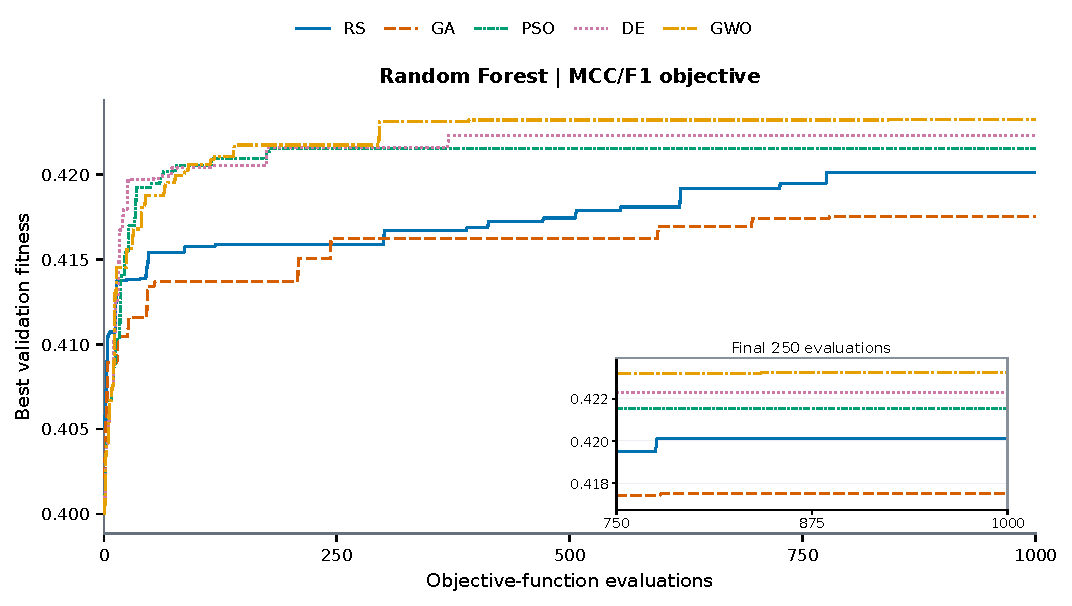
\includegraphics[width=0.91\linewidth]{figures/rf_convergence_mccf1.pdf}
\caption{Fitness evolution during equal-budget optimization of the Random Forest (RF) model under the MCC/$F_1$ validation objective. Lines show mean best-so-far fitness across the three common seeds. The y-axis is tightly scaled to the observed range; the inset magnifies the final 250 objective evaluations.}
\label{fig:rf_convergence_mccf1}\end{figure}

\begin{figure}[!htbp]\centering
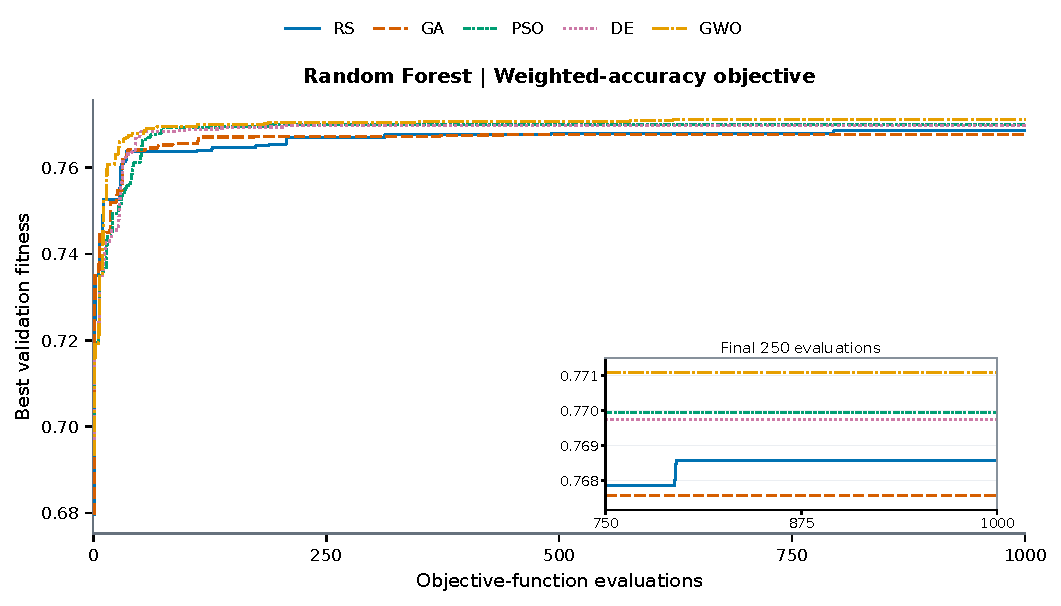
\includegraphics[width=0.91\linewidth]{figures/rf_convergence_accuracy.pdf}
\caption{Fitness evolution during equal-budget optimization of the Random Forest (RF) model under the weighted-accuracy validation objective. Lines show mean best-so-far fitness across the three common seeds. The y-axis is tightly scaled to the observed range; the inset magnifies the final 250 objective evaluations.}
\label{fig:rf_convergence_accuracy}\end{figure}

The RF panels differ mainly in the extent of late refinement: the MCC/$F_1$ trajectories retain somewhat more separation, whereas weighted-accuracy fitness ends in a tightly grouped set. Neither panel suggests a large payoff from spending the entire budget after the initial gains.

\subsubsection{Support Vector Machine}

Figures~\ref{fig:svm_convergence_mccf1} and~\ref{fig:svm_convergence_accuracy} display the strongest optimizer sensitivity. Under MCC/$F_1$, GWO and PSO make larger later gains and finish above RS and DE, while GA levels off at a lower fitness. Under weighted accuracy, GWO, PSO, and RS form a close upper group, DE finishes lower, and GA is lowest. These distinctions remain visible in the terminal insets, despite a common evaluation budget.

\begin{figure}[!htbp]\centering
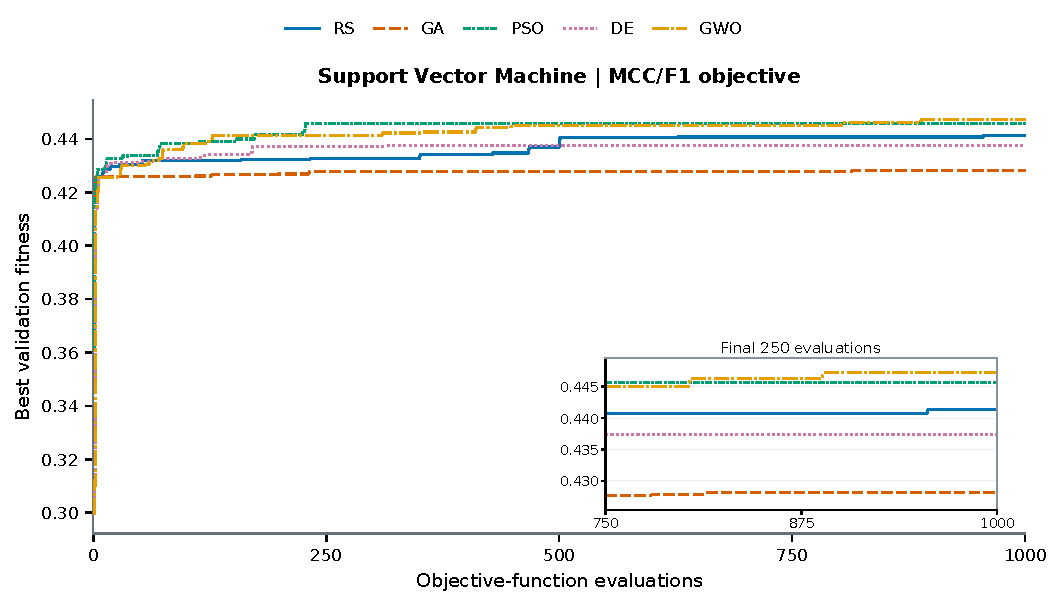
\includegraphics[width=0.91\linewidth]{figures/svm_convergence_mccf1.pdf}
\caption{Fitness evolution during equal-budget optimization of the support vector machine (SVM) under the MCC/$F_1$ validation objective. Lines show mean best-so-far fitness across the three common seeds. The y-axis is tightly scaled to the observed range; the inset magnifies the final 250 objective evaluations.}
\label{fig:svm_convergence_mccf1}\end{figure}

\begin{figure}[!htbp]\centering
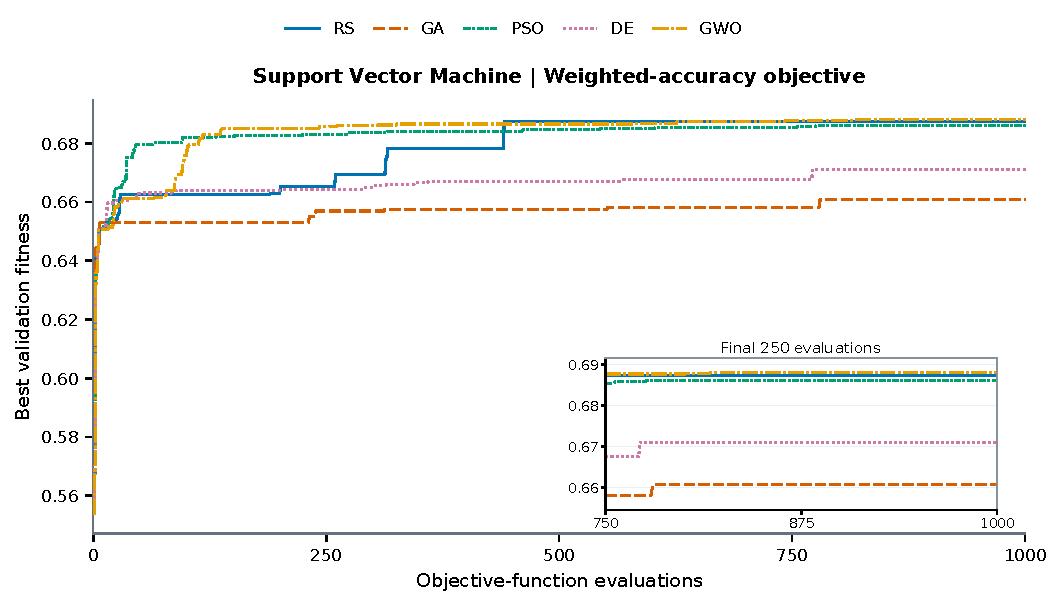
\includegraphics[width=0.91\linewidth]{figures/svm_convergence_accuracy.pdf}
\caption{Fitness evolution during equal-budget optimization of the support vector machine (SVM) under the weighted-accuracy validation objective. Lines show mean best-so-far fitness across the three common seeds. The y-axis is tightly scaled to the observed range; the inset magnifies the final 250 objective evaluations.}
\label{fig:svm_convergence_accuracy}\end{figure}
\FloatBarrier

This search sensitivity is consistent with the wide SVM locked-test dispersion in Table~\ref{tab:predictive_summary}. However, validation ranking does not determine the test ranking: under MCC/$F_1$, GA has the largest mean test MCC (0.290), although its validation-fitness trajectory finishes below GWO and PSO. Under weighted accuracy, GWO leads both the validation trajectory and the test-accuracy means, an alignment observed here rather than a general guarantee.

\subsubsection{Multilayer Perceptron}

Figures~\ref{fig:mlp_convergence_mccf1} and~\ref{fig:mlp_convergence_accuracy} reveal objective-dependent behaviour. With MCC/$F_1$ fitness, DE, PSO, GA, and GWO largely flatten during the later budget, whereas RS continues to improve and finishes above the other curves. That visual validation advantage does not carry through to locked-test MCC: RS averages 0.106, compared with 0.305 for GWO and 0.302 for DE in Table~\ref{tab:optimizer_primary_metrics}. Under weighted-accuracy fitness, all five trajectories become tightly clustered after their early gains and remain nearly indistinguishable near termination.

\begin{figure}[!htbp]\centering
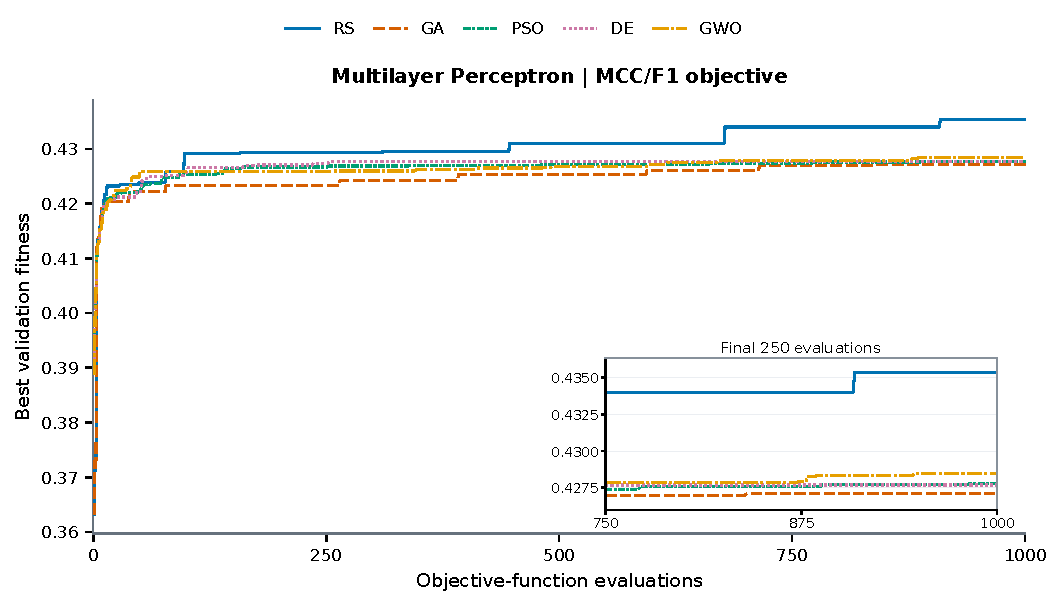
\includegraphics[width=0.91\linewidth]{figures/mlp_convergence_mccf1.pdf}
\caption{Fitness evolution during equal-budget optimization of the multilayer perceptron (MLP) under the MCC/$F_1$ validation objective. Lines show mean best-so-far fitness across the three common seeds. The y-axis is tightly scaled to the observed range; the inset magnifies the final 250 objective evaluations.}
\label{fig:mlp_convergence_mccf1}\end{figure}

\begin{figure}[!htbp]\centering
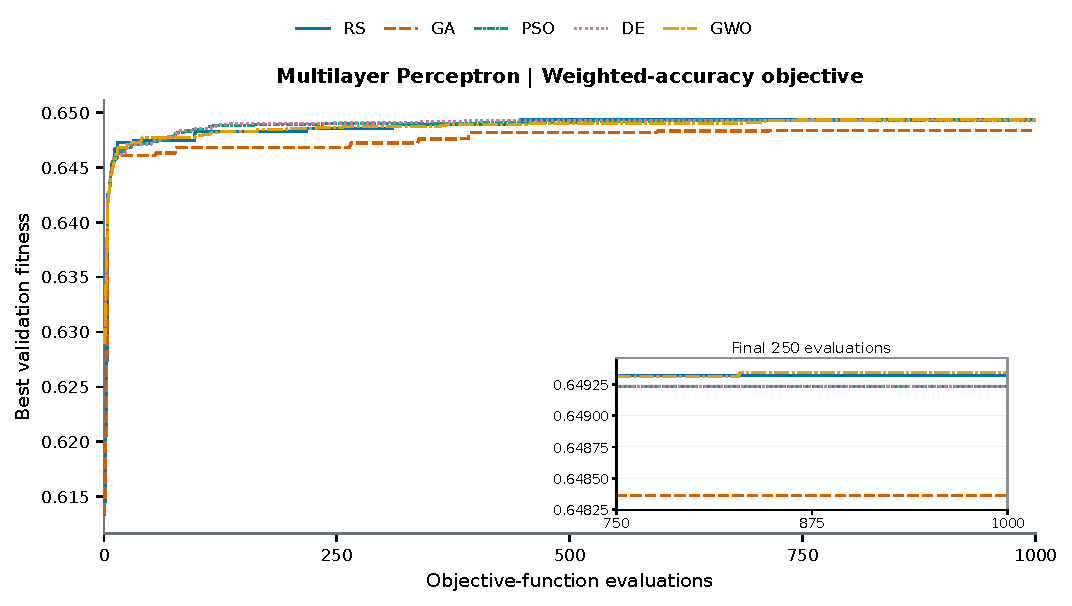
\includegraphics[width=0.91\linewidth]{figures/mlp_convergence_accuracy.pdf}
\caption{Fitness evolution during equal-budget optimization of the multilayer perceptron (MLP) under the weighted-accuracy validation objective. Lines show mean best-so-far fitness across the three common seeds. The y-axis is tightly scaled to the observed range; the inset magnifies the final 250 objective evaluations.}
\label{fig:mlp_convergence_accuracy}\end{figure}

The MLP curves show why visually similar terminal validation fitness must not be treated as identical generalization: under weighted accuracy, the locked-test means still span optimizer-specific values, while the MCC/$F_1$ panel's late RS advantage is paired with the lowest RS test MCC. These descriptive contrasts indicate that the objective shapes the selected search region, but do not establish why a particular configuration generalizes better.

\subsubsection{One-Dimensional Convolutional Neural Network}

Figures~\ref{fig:cnn_convergence_mccf1} and~\ref{fig:cnn_convergence_accuracy} show rapid early progress followed by a stable tail. Under MCC/$F_1$, PSO and GWO end at the upper edge of a compact group; GA and DE level off slightly lower, and RS lies between them. Under weighted accuracy, trajectories are again close after the initial rise, with GWO finishing marginally above the others. Relative to SVM, optimizer separation is narrower, especially for the weighted-accuracy trajectory.

\begin{figure}[!htbp]\centering
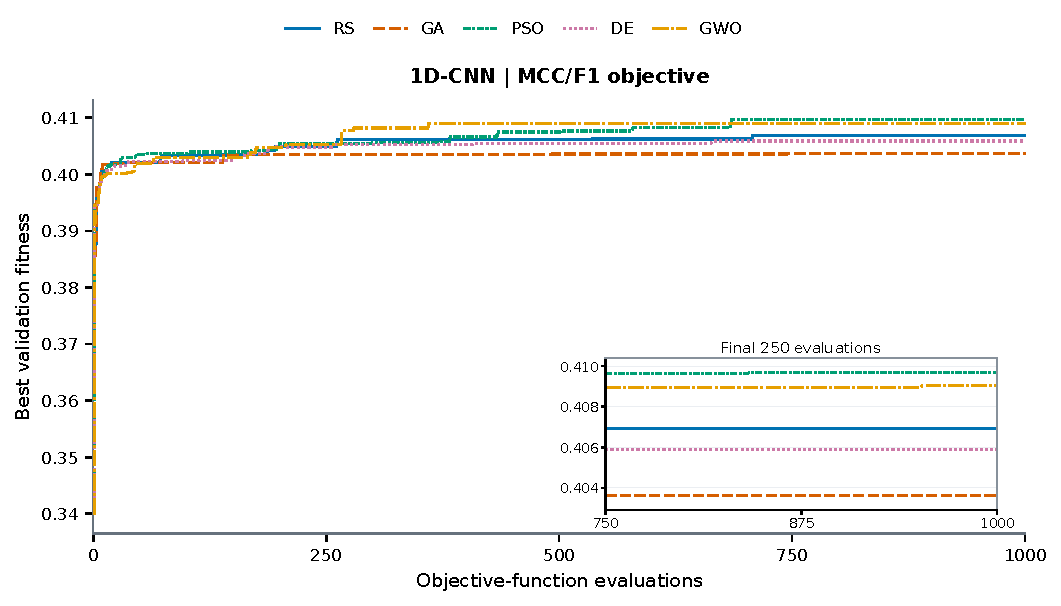
\includegraphics[width=0.91\linewidth]{figures/cnn_convergence_mccf1.pdf}
\caption{Fitness evolution during equal-budget optimization of the one-dimensional convolutional neural network (1D-CNN) under the MCC/$F_1$ validation objective. Lines show mean best-so-far fitness across the three common seeds. The y-axis is tightly scaled to the observed range; the inset magnifies the final 250 objective evaluations.}
\label{fig:cnn_convergence_mccf1}\end{figure}

\begin{figure}[!htbp]\centering
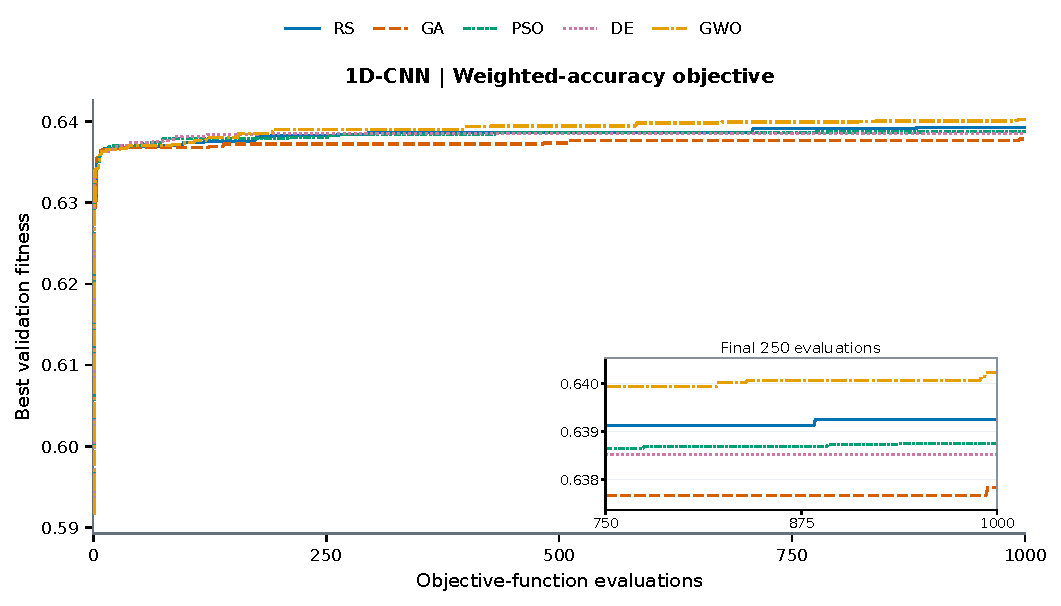
\includegraphics[width=0.91\linewidth]{figures/cnn_convergence_accuracy.pdf}
\caption{Fitness evolution during equal-budget optimization of the one-dimensional convolutional neural network (1D-CNN) under the weighted-accuracy validation objective. Lines show mean best-so-far fitness across the three common seeds. The y-axis is tightly scaled to the observed range; the inset magnifies the final 250 objective evaluations.}
\label{fig:cnn_convergence_accuracy}\end{figure}
\FloatBarrier

The test table qualifies these small validation gaps. Under MCC/$F_1$, PSO has the largest mean test MCC (0.269), while GWO's test MCC is 0.139 despite its near-leading validation trajectory. Under weighted accuracy, GWO also has the largest mean test accuracy (0.637), but the other four means are close (0.634--0.636). These are descriptive contrasts across three seeds, not evidence that a convergence curve identifies a statistically superior optimizer. Validation-fitness convergence measures search behaviour on development data; the locked chronological test block provides the relevant generalization comparison below.

\FloatBarrier

\subsection{Optimizer-Level Performance Under Equal Budget}

Convergence describes selection on validation fitness, not performance on the held-out period. Table~\ref{tab:optimizer_primary_metrics} therefore compares the locked-test endpoint aligned with each validation protocol: MCC for MCC/$F_1$ selection and accuracy for weighted-accuracy selection. Entries are means over three common seeds under the same 1,000-evaluation budget; they are descriptive summaries, not tests of optimizer superiority.

\begin{table}[htbp]
\centering
\caption{Optimizer-level locked-test primary metrics under equal budget. Each cell is a mean over three common seeds; boldface denotes the largest mean within a model and protocol. RS: Random Search; GA: Genetic Algorithm; PSO: Particle Swarm Optimization; DE: Differential Evolution; GWO: Grey Wolf Optimizer.}
\label{tab:optimizer_primary_metrics}
\footnotesize
\begin{tabular}{lccccc}\toprule
\textbf{Model} & \textbf{RS} & \textbf{GA} & \textbf{PSO} & \textbf{DE} & \textbf{GWO}\\\midrule
\multicolumn{6}{c}{\textbf{Panel A: MCC/$F_1$ fitness; locked-test MCC}}\\\midrule
RF & 0.281 & \textbf{0.293} & 0.293 & 0.292 & 0.288\\
SVM & 0.105 & \textbf{0.290} & 0.255 & 0.187 & 0.232\\
MLP & 0.106 & 0.290 & 0.299 & 0.302 & \textbf{0.305}\\
1D-CNN & 0.179 & 0.268 & \textbf{0.269} & 0.267 & 0.139\\\midrule
\multicolumn{6}{c}{\textbf{Panel B: weighted-accuracy fitness; locked-test accuracy}}\\\midrule
RF & 0.604 & \textbf{0.611} & 0.604 & 0.600 & 0.602\\
SVM & 0.588 & 0.557 & 0.571 & 0.584 & \textbf{0.593}\\
MLP & 0.649 & 0.649 & \textbf{0.652} & 0.652 & 0.652\\
1D-CNN & 0.636 & 0.634 & 0.635 & 0.634 & \textbf{0.637}\\\bottomrule
\end{tabular}
\end{table}

The table shows an optimizer-by-model interaction rather than a common winner. Under MCC/$F_1$, RF is comparatively insensitive among GA, PSO, and DE (0.293, 0.293, and 0.292), whereas its RS mean is 0.281. SVM is more sensitive: GA reaches 0.290, but RS reaches only 0.105; for MLP, GWO is highest at 0.305 while RS is again 0.106. The 1D-CNN is tightly grouped across GA, PSO, and DE (0.267--0.269), but lower for RS and particularly GWO. Under weighted-accuracy selection, the five MLP means are tightly clustered (0.649--0.652); the SVM range is wider (0.557--0.593), while RF spans 0.600--0.611 and 1D-CNN spans 0.634--0.637. Thus, optimizer sensitivity depends on both the backbone and the selected endpoint. With only three common seeds, the within-row maxima are not evidence of a universally best optimizer; the aggregated model comparison asks instead whether these patterns alter the backbone-level picture.

\subsection{Model-Level Aggregation Across Optimizers}

Table~\ref{tab:predictive_summary} and Figure~\ref{fig:model_comparison} jointly summarize the locked-test outcomes over 15 optimizer--seed blocks per backbone and protocol. The table retains dispersion across those blocks; the figure makes the change in model ordering between validation objectives easier to see. These are aggregate descriptions of the evaluated search procedures, not 15 independent market replications.

\begin{table}[!htbp]
\centering
\caption{Locked-test predictive outcomes by backbone and validation protocol. Entries are mean $\pm$ standard deviation over 15 optimizer--seed blocks per row (five optimizers $\times$ three common seeds).}
\label{tab:predictive_summary}
\small
\setlength{\tabcolsep}{7pt}
\begin{tabular}{lrrr}\toprule
\multicolumn{4}{c}{\textbf{Panel A: MCC/$F_1$ validation fitness}}\\\midrule
\textbf{Model} & Accuracy & MCC & $F_1$\\\midrule
RF & $0.645\pm0.004$ & $0.289\pm0.008$ & $0.664\pm0.006$\\
SVM & $0.604\pm0.060$ & $0.214\pm0.132$ & $0.602\pm0.122$\\
MLP & $0.630\pm0.070$ & $0.261\pm0.141$ & $0.639\pm0.071$\\
1D-CNN & $0.613\pm0.056$ & $0.224\pm0.120$ & $0.597\pm0.166$\\\midrule
\multicolumn{4}{c}{\textbf{Panel B: Weighted-accuracy validation fitness}}\\\midrule
\textbf{Model} & Accuracy & MCC & $F_1$\\\midrule
RF & $0.604\pm0.005$ & $0.208\pm0.009$ & $0.624\pm0.004$\\
SVM & $0.578\pm0.028$ & $0.159\pm0.053$ & $0.600\pm0.071$\\
MLP & $0.651\pm0.003$ & $0.301\pm0.005$ & $0.658\pm0.004$\\
1D-CNN & $0.635\pm0.002$ & $0.271\pm0.005$ & $0.639\pm0.007$\\\bottomrule
\end{tabular}
\end{table}

In Panel A of Table~\ref{tab:predictive_summary}, RF has the highest aggregate mean for accuracy, MCC, and $F_1$, and its standard deviations are small (0.004, 0.008, and 0.006). SVM, MLP, and 1D-CNN show appreciably larger dispersion, especially for MCC/$F_1$ selection. Panel B reverses the leading backbone: MLP has the highest mean across all three metrics and low dispersion; 1D-CNN is also competitive, while RF's mean accuracy and MCC are lower than in Panel A. The pattern suggests that the validation objective changes which model/configuration regions the search favours; it does not establish that either objective is globally superior.

\begin{figure}[!htbp]\centering
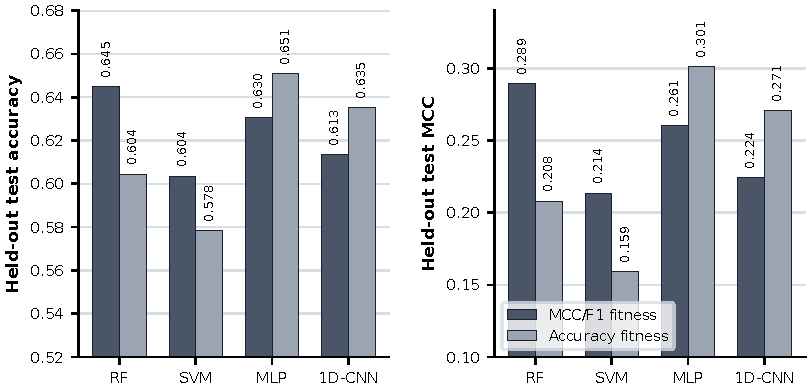
\includegraphics[width=0.94\linewidth]{figures/ijcnn_style_model_performance.pdf}
\caption{Mean locked-test accuracy and MCC for four model families under the two validation objectives, aggregated over 15 optimizer--seed blocks per model and protocol.}
\label{fig:model_comparison}\end{figure}

Figure~\ref{fig:model_comparison} makes this objective-dependent ordering visible: RF leads the MCC/$F_1$ panel-level means, whereas MLP leads under weighted-accuracy selection, with 1D-CNN close behind MLP on weighted-accuracy test accuracy. The figure's grouped bars show means, while Table~\ref{tab:predictive_summary} supplies the dispersion needed to judge stability. Accuracy and MCC are complementary here: a change in overall correct classifications need not preserve the model's class-balanced association, so neither panel should be reduced to one endpoint. These differences are meaningful as descriptions of this locked interval, but the single chronological test period limits claims about future market regimes.

\subsection{Exploratory Statistical Evidence}

Table~\ref{tab:predictive_inference} reports exploratory Friedman comparisons of the four backbones within each protocol. In each of the 15 blocks (five optimizers crossed with three seeds), the backbones are ranked on the protocol-aligned locked-test endpoint; the Friedman statistic assesses whether those within-block rankings are uniform. The stacked panels keep each global test beside the corresponding backbone mean ranks.

\begin{table}[!htbp]
\centering
\caption{Exploratory Friedman tests for protocol-aligned locked-test endpoints across four backbones. Each test uses 15 matched optimizer--seed blocks from the same chronological test interval. Mean ranks are block-wise; lower is better.}
\label{tab:predictive_inference}
\small
\setlength{\tabcolsep}{6pt}
\begin{tabular}{lrrr}\toprule
\multicolumn{4}{c}{\textbf{Panel A: MCC/$F_1$ fitness}}\\\midrule
Endpoint & $n$ & $\chi^2$ & $p$\\\midrule
Test MCC & 15 & 22.84 & $4.36\times10^{-5}$\\\bottomrule
\end{tabular}

\vspace{0.45em}
\begin{tabular}{lrrrr}\toprule
\multicolumn{5}{c}{\textbf{Mean ranks (lower is better)}}\\\midrule
Model & RF & SVM & MLP & 1D-CNN\\\midrule
Mean rank & 2.07 & 2.73 & 1.53 & 3.67\\\bottomrule
\end{tabular}

\vspace{0.8em}
\begin{tabular}{lrrr}\toprule
\multicolumn{4}{c}{\textbf{Panel B: Weighted-accuracy fitness}}\\\midrule
Endpoint & $n$ & $\chi^2$ & $p$\\\midrule
Test accuracy & 15 & 42.92 & $2.56\times10^{-9}$\\\bottomrule
\end{tabular}

\vspace{0.45em}
\begin{tabular}{lrrrr}\toprule
\multicolumn{5}{c}{\textbf{Mean ranks (lower is better)}}\\\midrule
Model & RF & SVM & MLP & 1D-CNN\\\midrule
Mean rank & 3.13 & 3.87 & 1.00 & 2.00\\\bottomrule
\end{tabular}
\end{table}

Under MCC/$F_1$, the Friedman test detects differences in matched-block ordering ($\chi^2=22.84$, $p=4.36\times10^{-5}$). RF has the largest marginal mean MCC in Table~\ref{tab:predictive_summary}, while MLP has the lowest mean rank in Table~\ref{tab:predictive_inference}; this is not contradictory. A marginal mean aggregates score magnitudes across blocks, whereas the mean rank first orders the backbones separately within each block and then averages those ranks. A model can therefore rank consistently well without having the largest pooled score magnitude. Under weighted accuracy, MLP leads both the mean accuracy and mean rank; the reported Holm-adjusted contrasts against RF, SVM, and 1D-CNN are significant ($p_{\mathrm{Holm}}\approx0.00194$) within this analysis.

These results remain exploratory. The 15 blocks are optimizer--seed combinations on one shared chronological market interval, not 15 independent market replications. The tests describe consistency across the evaluated search combinations; they do not establish replication across regimes or a confirmatory difference between validation objectives. Their interpretation should remain paired with the descriptive dispersion in Table~\ref{tab:predictive_summary}.

\subsection{Exploratory Economic Evaluation}

Table~\ref{tab:economic_summary} and Figure~\ref{fig:economic_comparison} compare return and downside risk under the fixed intrabar execution rule. The table reports net profit and maximum drawdown with dispersion, alongside mean profit factor and annualized Sharpe; the figure places mean return against mean drawdown. This joint view is important because total profit alone does not represent a complete return--risk profile.

\begin{table}[!htbp]
\centering
\caption{Exploratory economic outcomes under the fixed intrabar execution rule, aggregated over 15 optimizer--seed blocks per model and protocol. Net profit and maximum drawdown (Max. DD) are points and reported as mean $\pm$ standard deviation; PF and annualized Sharpe are means.}
\label{tab:economic_summary}
\footnotesize
\begin{tabular}{llrrrr}\toprule
\textbf{Protocol} & \textbf{Model} & \textbf{Net profit} & \textbf{Max. DD} & \textbf{PF} & \textbf{Sharpe}\\\midrule
\multirow{4}{*}{MCC/$F_1$ fitness} & RF & $26{,}465\pm1{,}732$ & $-2{,}126\pm141$ & 1.48 & 12.50\\
& SVM & $17{,}017\pm29{,}437$ & $-9{,}823\pm17{,}123$ & 1.39 & 8.52\\
& MLP & $22{,}110\pm20{,}556$ & $-5{,}503\pm12{,}984$ & 1.43 & 10.62\\
& 1D-CNN & $19{,}969\pm17{,}574$ & $-5{,}991\pm10{,}469$ & 1.37 & 7.67\\\midrule
\multirow{4}{*}{Weighted accuracy fitness} & RF & $21{,}973\pm1{,}336$ & $-1{,}866\pm365$ & 1.38 & 11.95\\
& SVM & $11{,}440\pm13{,}350$ & $-5{,}241\pm1{,}961$ & 1.21 & 4.18\\
& MLP & $27{,}737\pm1{,}069$ & $-2{,}141\pm112$ & 1.51 & 13.07\\
& 1D-CNN & $26{,}861\pm1{,}924$ & $-2{,}494\pm62$ & 1.49 & 9.71\\\bottomrule
\end{tabular}
\end{table}

\begin{figure}[!htbp]\centering
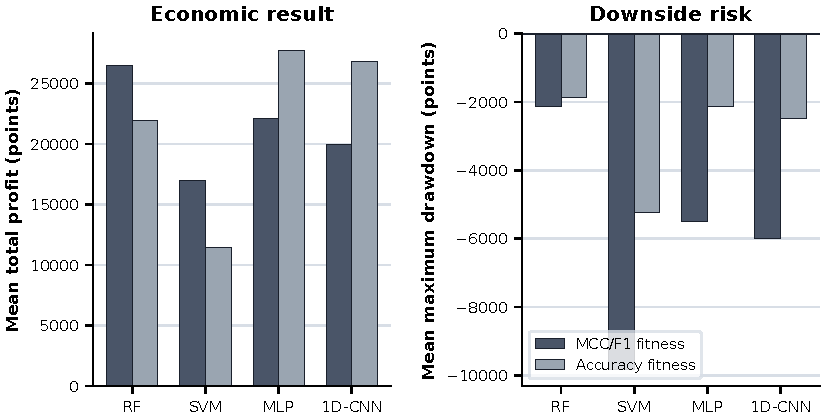
\includegraphics[width=0.94\linewidth]{figures/ijcnn_style_economic_summary.pdf}
\caption{Mean total profit and mean maximum drawdown across 15 optimizer--seed blocks per model and validation protocol. Both axes are in points; a drawdown closer to zero indicates a smaller loss peak-to-trough.}
\label{fig:economic_comparison}\end{figure}

The return--risk comparison in Figure~\ref{fig:economic_comparison} shows the protocol-dependent change in mean profit and drawdown, while Table~\ref{tab:economic_summary} adds the other endpoints. Under MCC/$F_1$, RF combines the largest mean net profit (26,465 points) with PF 1.48, Sharpe 12.50, and a comparatively small mean drawdown (-2,126 points) with SD 141. Under weighted accuracy, MLP has the largest mean profit (27,737 points), PF 1.51, and Sharpe 13.07; RF instead has the least negative mean drawdown (-1,866 points). The metric leader therefore depends on which component of return and risk is prioritized, and the most profitable mean is not by itself a complete ranking. These backtest summaries are exploratory under the specified rule and costs, not a trading recommendation or a transaction-cost-complete assessment.

Appendix~\ref{app:benchmark_visualizations} provides complementary views. Figures~\ref{fig:heatmap_mccf1_mcc_test} and~\ref{fig:heatmap_accuracy_accuracy_test} show how the optimizer-by-model pattern depends on protocol; Figure~\ref{fig:test_mcc_seed_boxplots} exposes seed-level MCC dispersion hidden by cell means. Figure~\ref{fig:optimizer_average_ranks} summarizes optimizer ordering descriptively, Figure~\ref{fig:performance_vs_fit_time} displays the performance--candidate-fit-time trade-off, and Figure~\ref{fig:benchmark_radar} gives a normalized multi-metric overview. These supplementary plots help locate patterns but do not replace the tables or extend the inferential scope of the single-period experiment.
